%% FEUP THESIS STYLE for LaTeX2e
%% how to use feupteses (English version)
%%
%% FEUP, JCL & JCF, 31 July 2012
%%
%% PLEASE send improvements to jlopes at fe.up.pt and to jcf at fe.up.pt
%%

%%========================================
%% Commands: pdflatex tese
%%           bibtex tese
%%           makeindex tese (only if creating an index)
%%           pdflatex tese
%% Alternative:
%%          latexmk -pdf tese.tex
%%========================================

\documentclass[11pt,a4paper,twoside,openright]{report}

%% For iso-8859-1 (latin1), comment next line and uncomment the second line
\usepackage[utf8]{inputenc}
%\usepackage[latin1]{inputenc}

%% English version

%% MIEIC options
\usepackage[mieic]{feupteses}
%\usepackage[mieic,juri]{feupteses}
%\usepackage[mieic,final]{feupteses}
%\usepackage[mieic,final,onpaper]{feupteses}

% For gantt timeline diagrams
\usepackage{pgfgantt}

\usepackage{cite}
\usepackage{makeidx}
\usepackage[utf8]{inputenc}
\usepackage{multirow}
\usepackage{graphicx}
\usepackage[acronym]{glossaries}

%%% For charts%%
\usepackage{tikz}

%% For code block %%
\usepackage{listings}
\lstset{basicstyle=\footnotesize\ttfamily,breaklines=true}
\lstset{framextopmargin=0pt,frame=lrbt,rulecolor=\color{Gray}}
%%%

\newcommand{\apiname}{SAJaS} 
\newcommand{\apilongname}{Simple API for JADE-based Simulations}

%!TEX root = doc.tex

\title{\LARGE \bf
Bridging the Gap between MAS Simulation and Development using a JADE-based API for Repast
}


\author{João P. C. Lopes,
	Henrique Lopes Cardoso,
	João S. V. Gonçalves %
}

\institute{
		DEI, Faculdade de Engenharia, Universidade do Porto \\
		Porto, Portugal \\
		LIACC -- Laboratório de Inteligência Artificial e Ciência de Computadores \\
		Porto, Portugal \\
        \{lopes.joao.pedro, hlc, joao.sa.vinhas\}@fe.up.pt %
}


% Acronym definitions (doesn't render acronyms page)
% format: \newacronym{<label>}{<abbrv>}{<full>}

%% Acronyms and Abreviations

\newacronym{ACL}{ACL}{Agent Communication Language}
\newacronym{AMS}{AMS}{Agent Management System}
\newacronym{AST}{AST}{Abstract Syntax Tree}
\newacronym{ATL}{ATL}{ATLAS Transformation Language}
\newacronym{CeCILL-C}{CeCILL-C}{CEA CNRS INRIA Logiciel Libre (open source license)}
\newacronym{DF}{DF}{Directory Facilitator}
\newacronym{EPL}{EPL}{Eclipse Public License (open source license)}
\newacronym{FIPA}{FIPA}{The Foundation for Intelligent Physical Agents}
\newacronym{FOSS}{FOSS}{Free and Open Source Software}
\newacronym{IDE}{IDE}{Integrated Development Environment}
\newacronym{JADE}{JADE}{Java Agent DEvelopment Framework}
\newacronym{JDT}{JDT}{[Eclipse] Java Development Tools}
\newacronym{MABS}{MABS}{Multi-Agent-Based Simulation}
\newacronym{MAS}{MAS}{Multi-Agent System}
\newacronym{MTS}{MTS}{Message Transport Service}

\newacronym{Repast}{Repast}{Recursive Porous Agent Simulation Toolkit}

%% Additional options for feupteses.sty: 
%% - onpaper: links are not shown (for paper versions)
%% - backrefs: include back references from bibliography to citation place

%% Uncomment the next lines if side by side graphics used
%\usepackage[lofdepth,lotdepth]{subfig}
%\usepackage{graphicx}
%\usepackage{float}

%% Include color package
\usepackage{color}
\definecolor{Highlight}{rgb}{0.8,0.8,0.0}

%% Include source-code listings package
\usepackage{listings}
\lstset{ %
 language=C,                        % choose the language of the code
 basicstyle=\footnotesize\ttfamily,
 keywordstyle=\bfseries,
 numbers=left,                      % where to put the line-numbers
 numberstyle=\scriptsize\texttt,    % the size of the fonts that are used for the line-numbers
 stepnumber=1,                      % the step between two line-numbers. If it's 1 each line will be numbered
 numbersep=8pt,                     % how far the line-numbers are from the code
 frame=tb,
 float=htb,
 aboveskip=8mm,
 belowskip=4mm,
 backgroundcolor=\color{cloudwhite},
 showspaces=false,                  % show spaces adding particular underscores
 showstringspaces=false,            % underline spaces within strings
 showtabs=false,                    % show tabs within strings adding particular underscores
 tabsize=2,                     % sets default tabsize to 2 spaces
 captionpos=b,                      % sets the caption-position to bottom
 breaklines=true,                   % sets automatic line breaking
 breakatwhitespace=false,           % sets if automatic breaks should only happen at whitespace
 escapeinside={\%*}{*)},            % if you want to add a comment within your code
 morekeywords={*,var,template,new}  % if you want to add more keywords to the set
}

%% Uncomment to create an index (at the end of the document)
%\makeindex

%% Path to the figures directory
%% TIP: use folder ``figures'' to keep all your figures
\graphicspath{{figures/}}



%%========================================
%% Start of document
%%========================================
\begin{document}

%%----------------------------------------
%% Information about the work
%%----------------------------------------
\title{From simulation to development in MAS: Repast-JADE automatic code generation for interaction protocols}
\author{João Pedro Camacho Lopes}

%% Uncomment next line for date of submission
%\thesisdate{July 31, 2008}

%%Uncomment next line for copyright text if used
%\copyrightnotice{Name of the Author, 2008}

\supervisor{Supervisor}{Henrique Lopes Cardoso}

%% Uncomment next line if necessary
%\supervisor{Second Supervisor}{Name of the Supervisor}

%% Uncomment committee stuff in the final version if used
%\committeetext{Approved in oral examination by the committee:}
%\committeemember{Chair}{Doctor Name of the President}
%\committeemember{External Examiner}{Doctor Name of the Examiner}
%\committeemember{Supervisor}{Doctor Name of the Supervisor}
%\signature

%% Specify cover logo (in folder ``figures'')
\logo{uporto-feup.pdf}

%% Uncomment next line for additional text  below the author's name (front page)
\additionalfronttext{}

%%----------------------------------------
%% Preliminary materials
%%----------------------------------------

% remove unnecssary \include{} commands
\begin{Prolog}
  %!TEX root = doc.tex

\begin{abstract}

% 1 - Intro
Agent-based applications and simulations are in widespread use today in both research and industry.
\gls{MAS} and \gls{MABS} are two approaches to make use of multi-agent systems technology, each with distinct characteristics and goals.
% 2 - Problem
While open agent-based applications benefit from adopting interaction standards, most \gls{MABS} frameworks do not support them.
% 3 - Proposal 
In this paper we propose an architecture, based on FIPA and JADE, for agent-based simulations, focusing on supporting agent communication using FIPA interaction protocols.
Based on this architecture, we present the \apiname{} API, whose goal is to bring JADE and Repast, two popular \gls{MAS} and \gls{MABS} development frameworks, closer together, facilitating the creation of simulations by JADE programmers and enabling an automatic portability between both frameworks.
% 4 - Experimentation/Validation
For illustration, we show the creation of a simulation where agents interact in a contract net.
Finally, we present an early overview of a code conversion tool whose aim is to automatically generate a JADE \gls{MAS} from a Repast simulation that makes use of \apiname{}.
% 5 - Conclusions?
%%
%% TODO
%%
\glsresetall
\end{abstract}

%\begin{IEEEkeywords}
%
%\end{IEEEkeywords}
 % the abstract
  % \chapter*{Acknowledgements}

Aliquam id dui. Nulla facilisi. Nullam ligula nunc, viverra a, iaculis
at, faucibus quis, sapien. Cum sociis natoque penatibus et magnis dis
parturient montes, nascetur ridiculus mus. Curabitur magna ligula,
ornare luctus, aliquam non, aliquet at, tortor. Donec iaculis nulla
sed eros. Sed felis. Nam lobortis libero. Pellentesque
odio. Suspendisse potenti. Morbi imperdiet rhoncus magna. Morbi
vestibulum interdum turpis. Pellentesque varius. Morbi nulla urna,
euismod in, molestie ac, placerat in, orci. 

Ut convallis. Suspendisse luctus pharetra sem. Sed sit amet mi in diam
luctus suscipit. Nulla facilisi. Integer commodo, turpis et semper
auctor, nisl ligula vestibulum erat, sed tempor lacus nibh at
turpis. Quisque vestibulum pulvinar justo. Class aptent taciti
sociosqu ad litora torquent per conubia nostra, per inceptos
himenaeos. Nam sed tellus vel tortor hendrerit pulvinar. Phasellus
eleifend, augue at mattis tincidunt, lorem lorem sodales arcu, id
volutpat risus est id neque. Phasellus egestas ante. Nam porttitor
justo sit amet urna. Suspendisse ligula nunc, mollis ac, elementum
non, venenatis ut, mauris. Mauris augue risus, tempus scelerisque,
rutrum quis, hendrerit at, nunc. Nulla posuere porta orci. Nulla dui. 

Fusce gravida placerat sem. Aenean ipsum diam, pharetra vitae, ornare
et, semper sit amet, nibh. Nam id tellus. Etiam ultrices. Praesent
gravida. Aliquam nec sapien. Morbi sagittis vulputate dolor. Donec
sapien lorem, laoreet egestas, pellentesque euismod, porta at,
sapien. Integer vitae lacus id dui convallis blandit. Mauris non
sem. Integer in velit eget lorem scelerisque vehicula. Etiam tincidunt
turpis ac nunc. Pellentesque a justo. Mauris faucibus quam id
eros. Cras pharetra. Fusce rutrum vulputate lorem. Cras pretium magna
in nisl. Integer ornare dui non pede. 

\vspace{10mm}
\flushleft{The Name of the Author}
  % the acknowledgments
  % \cleardoublepage
\thispagestyle{plain}

\vspace*{8cm}

\begin{flushright}
   \textsl{``You should be glad that bridge fell down. \\
           I was planning to build thirteen more to that same design''} \\
\vspace*{1.5cm}
           Isambard Kingdom Brunel
\end{flushright}
       % initial quotation if desired
  \cleardoublepage
  \pdfbookmark[0]{Table of Contents}{contents}
  \tableofcontents
  \cleardoublepage
  \pdfbookmark[0]{List of Figures}{figures}
  \listoffigures
  \cleardoublepage
  \pdfbookmark[0]{List of Tables}{tables}
  \listoftables
  %!TEX root = thesis.tex
\chapter*{Abbreviations}
\chaptermark{ABBREVIATIONS}

\begin{flushleft}
\begin{tabular}{l p{0.8\linewidth}}
ACL		 & Agent Communication Language \\
AST		 & Abstract Syntax Tree \\
ATL		 & ATLAS Transformation Language \\
CeCILL-C	& CEA CNRS INRIA Logiciel Libre (open source license) \\
EPL		 & Eclipse Public License (open source license) \\
FIPA	 & Foundation for Intelligent Physical Agents \\
FOSS 	 & Free and Open Source Software \\
IDE 	 & Integrated Development Environment \\
JADE	 & Java Agent DEvelopment Framework \\
JDT		 & [Eclipse] Java Development Tools \\
MABS	 & Multi-Agent-Based Simulation \\
MAS      & Multi-Agent System \\

\end{tabular}
\end{flushleft}

  % the list of abbreviations used
\end{Prolog}

%%----------------------------------------
%% Body
%%----------------------------------------
\StartBody

%% TIP: use a separate file for each chapter
%!TEX root = doc.tex
\section{Introduction} % (fold)
\label{sec:introduction}

% 1 - Intro to MAS
A \gls{MAS} is composed of autonomous intelligent agents, capable of interacting with each other \cite{wooldridge2008introduction}.
Agent-based applications are in widespread use in multiple fields of research and industry and can be heterogeneous, often requiring interoperation between agents from different systems.
In order to make this possible, agent technologies have matured and standards have emerged to support the interaction between agents.

% 2 - FIPA and ACL
The specifications of \gls{FIPA}\footnote{http://www.fipa.org/} promote interoperability in heterogeneous agent systems.
These standards define not only a common \gls{ACL}, but also a group of interaction protocols, recommended facilities for agent management and directory services \cite{o1998fipa}.

% 3 - Framework problems (not supporting FIPA)
Several frameworks exist \cite{survey,survey2} that offer some level of abstraction from low level development, allowing programmers to focus on a more conceptual approach in \gls{MAS} design.
% They are usually focused in one or more domains.
It turns out, though, that \gls{FIPA} standards (or any standards) are not supported by all of them.

% 4 - This paper focus JADE and Repast
In this paper we focus on two frameworks, the \gls{JADE} and the \gls{Repast}. For this paper, version 4.3.2 of JADE and version 2.1 of Repast Simphony (henceforth designated simply as ``Repast'') were used.

% 4.1 - \gls{JADE}
\gls{JADE} is a \gls{FIPA}-compliant, general-purpose (i.e. not focused on a single domain) framework used in the development of distributed agent applications.
It seamlessly hides all complexity concerning its distributed architecture \cite{bellifemine2003JADE}.
However, experiments with \gls{JADE} show that the platform's scalability is limited \cite{mengistu2008scalability}, meaning that \gls{JADE} is not an appropriate tool to create MABS which usually deal with a large number of agents.

% 4.2 - Repast
Repast, on the other hand, is a very rich simulation tool \cite{repSimph}, but does not support any open standards. Table \ref{tab:jadevsrep} summarizes the main differences between the two frameworks. One of the main motivations of the solution we propose is to enable Repast-based \gls{FIPA}-compliant simulations, thus making them more similar to distributed MAS implementations. This solution can be useful in scenarios where proficient JADE developers intend to create Repast simulations, allowing them to use familiar JADE-like tools. 
Furthermore, we wish to enable the conversion of Repast models into full featured \gls{JADE} MAS, as well as the conversion of \gls{JADE} MAS into Repast simulations, thus further closing the gap between the two frameworks.

\begin{table}[h]
	\normalsize
	\caption{Comparison of JADE and Repast features.}
	\label{tab:jadevsrep}
	\begin{center}
		\begin{tabular}{l|cc}
		\hline

		\hline
		\textbf{} & \textbf{JADE} & \textbf{Repast} \\ %& \textbf{Cougaar} \\
		\hline
			Agent 		& ACL  	&  Method calls  \\ %& Serialized Object \\
			Interaction	& Messages	&  Shared resources \\
		\hline
			Distribution & Yes & No \\ %& Yes \\
		\hline
			Simulation Tools & No & Yes \\ %& Yes \\
		\hline
			Scalability & Limited & High \\ %& High \\
		\hline
			Ontologies & Yes & No \\ %& Yes\\
		\hline
			Agent  		& Behavior-based & Schedule-based  \\ %&  \\
			Execution	& Multi-threaded & Single-threaded \\ %&  \\
						& Event-driven   & Tick-driven 	   \\ %&  \\
						& Assync		 & Sync 		   \\ %&  \\
		\hline
		\end{tabular}
	\end{center}
\end{table} 

% 5 - Proposal 
With these goals in mind, we propose the use of an API when developing Repast-based simulations. \apiname{} (\apilongname{}) addresses not only agent programming, but also their interaction and related infrastructural components.
We are aware that this kind of facilities is only valuable for true multi-agent based simulation, and not in general for any agent-based modelling and simulation approach (for which Repast is also suited).

% 6 - Challenges
Developing \apiname{} presented some challenges.
%Some of the challenges of developing this software lie in balancing its complexity.
MABS's execution is usually very fast paced; maintaining a simple architecture with a low impact on performance is therefore important.
The architecture we propose, however, is based on \gls{JADE}.
A compromise has been met by porting the features from \gls{JADE} that we find most valuable in a \gls{MAS} and that are needed for a meaningful exploitation of both frameworks.

% 7 - Objectives
One of the guidelines while developing this API was to make the software considerably generic, in the sense that it is not heavily dependent on a framework.
We accomplished this by using a pure Java implementation that does not rely on constructs provided by Repast or \gls{JADE}, as opposed to some of the similar works we discuss in Section \ref{sec:related_work}.
%% Related work
Those works try to integrate both frameworks in a single environment, seeking to use the best of \gls{JADE} and Repast. They are still relevant to our proposal since they give important insight on how to implement interaction protocols available in \gls{JADE} (inherently event-driven) in Repast's tick-based scheduler.

Section \ref{sec:fipa} contains a brief discussion about FIPA specifications, especially focused on the concepts present in JADE that are relevant to this project.
%% Architecture
The details of the API are defined in Section \ref{sec:proposal}. We provide a clear overview of its architecture and justify our design decisions and how it compares to \gls{JADE}'s own implementation.
%% Verification
For exemplification and comparison purposes, in Section \ref{sec:verification} we present an experiment performed in both frameworks and using \apiname{}.
%% Prototype
In Section \ref{sec:prototype} we present our proposal for the code conversion tool that will allow programmers to convert between Repast simulations created with \apiname{} and \gls{JADE} applications. While still under development, we try to give an overview of its main features.
% Conclusions
Finally, Section 7 concludes the paper and points future work.








%!TEX root = doc.tex
\section{Related Work} % (fold)
\label{sec:related_work}

%% Intro to the related work
Some works \cite{garcia2011misia,gormer2011jrep,YooG08,warden2010towards} have approached the problem of complementing Repast and JADE's features by using them together.
We chose to briefly describe two such approaches: MISIA and JRep. They propose combining Repast and \gls{JADE}, allowing the creation of Repast simulations that also take advantage of JADE's networking capabilities and use of \gls{FIPA} standards.

%% MISIA
\subsection{MISIA}
MISIA's approach, as suggested by Figure \ref{fig:misia}, is to use a middle layer that acts as the bridge between two other layers that interact with JADE and Repast Simphony.
By extending the agents in Repast and JADE, communicating through a coordinator and synchronizing their state, these agents work as a single one.

\begin{figure}
	\centering
	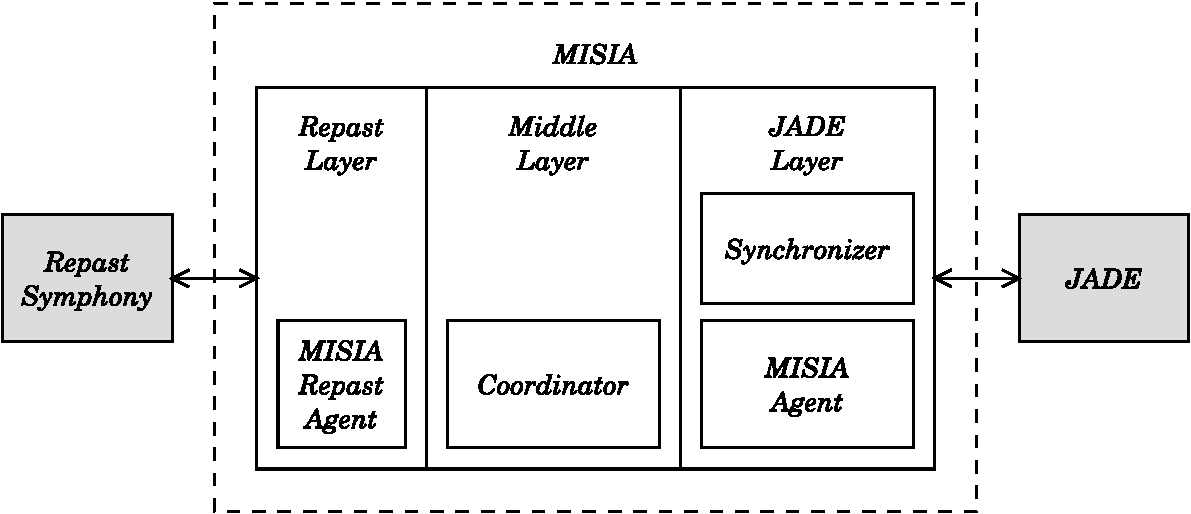
\includegraphics[width=3.0in]{figures/MISIA.pdf}
	\caption{High-level representation of MISIA's architecture (adapted from \cite{garcia2011misia})}
	\label{fig:misia}
\end{figure}

One of the challenges identified by the authors when re-implementing the FIPA interaction protocols was synchronizing them with the Repast tick-based simulation model.
Given JADE's event-driven architecture, MISIA proposes the use of a coordinator agent that informs the JADE-Agent when a tick has passed.
It also proposes its own implementation of the interaction protocols supported by JADE, making them tick-friendly.

%% JREP
\subsection{JRep}
JReps's approach is not as complex as MISIA's.
By having the Repast Simphony agent encapsulate a JADE agent representation, synchronization is immediate and is assured without requiring an external coordinator.
The two agent representations take care of synchronizing any state changes.
Figure \ref{fig:jrep} represents the basic structure of JRep.

\begin{figure}
	\centering
	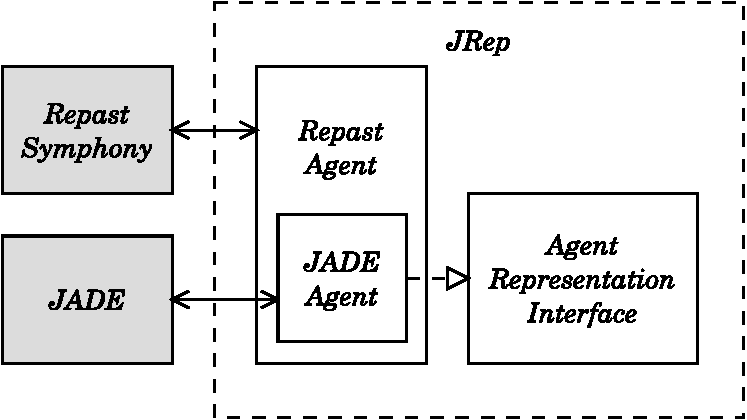
\includegraphics[width=2.1in]{figures/jrep.pdf}
	\caption{High-level representation of JRep's architecture}
	\label{fig:jrep}
\end{figure}

Each agent takes care of interfacing their respective frameworks. The interaction between agents in JRep is performed using FIPA ACL and the protocol implementations are those provided by the JADE platform. Similarly to MISIA, an Agent Representation Interface is used to introduce the concept of schedule in the JADE agent


%% COMPARISON
\subsection{Comparison with \apiname{}}

JADE is a very rich platform but, for many simulation scenarios, the overhead introduced by it has a significant impact on simulation performance \cite{mengistu2008scalability}. \apiname{}, as we describe with more detail in Section \ref{sec:proposal}, uses an architecture that is conceptually very close to JADE's but tailored for Repast with no extra dependencies. Moreover, the API could be used with other simulation frameworks with little adaptation.

As suggested by Figure \ref{fig:related-repacl}, \apiname{}'s general structure is simpler than that of JRep and MISIA. Our API does not intend to maintain an active connection to a JADE platform, eliminating the need for synchronization. Instead, our goal is to replicate in our API the main features of JADE, allowing for a straightforward and dependency free feature mapping between our API and JADE.

\begin{figure}
	\centering
	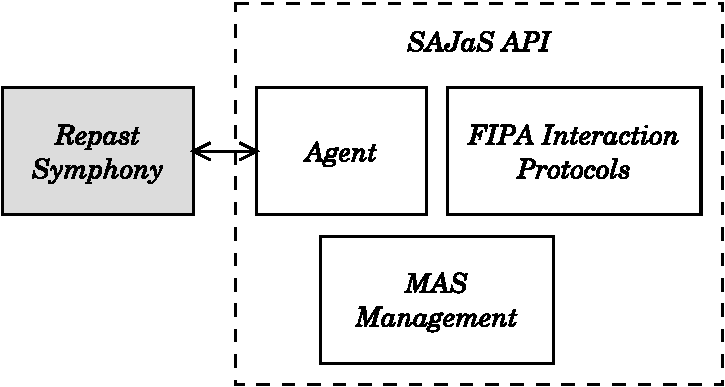
\includegraphics[width=2.1in]{figures/repacl.pdf}
	\caption{Basic structure of \apiname{}}
	\label{fig:related-repacl}
\end{figure}

In both MISIA and JRep, even though they attempt to integrate the features from both JADE and Repast, as far as Repast simulations are concerned JADE's multi-threaded infrastructure affects their performance very significantly. The main advantage of our approach is, therefore, the possibility of using Repast with JADE features, namely FIPA specifications including interaction protocols, without the need to interface with JADE. In Section \ref{sec:proposal} we provide a more detailed description of \apiname{}.


%!TEX root = doc.tex
\section{FIPA Specifications} % (fold)
\label{sec:fipa}

% Intro to FIPA in JADE/API
\apiname{} closely follows JADE's architecture regarding the use of protocols and services specified by \gls{FIPA}. The architecture of the API described in this paper includes multiple concepts proposed by \gls{FIPA}: the \gls{DF}, the \gls{MTS}, the \gls{AMS}, the \gls{ACL} Message and the Interaction Protocols. The following is a brief description of these concepts and of how JADE uses and implements them.

%\begin{figure}
%	\centering
%	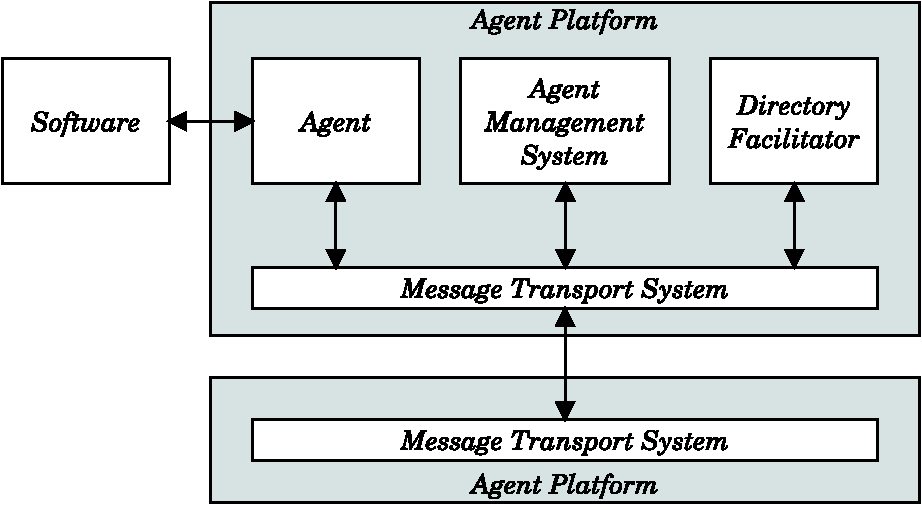
\includegraphics[width=2.5in]{figures/pdf/AMSdiagram.pdf}
%	\caption{
%		Agent Management Reference Model, as specified by FIPA and implemented by JADE. \apiname{} only supports a single Agent Platform.
%	}
%	\label{fig:AMSdiagram}
%\end{figure}

% DF 
The \gls{DF} is a component that provides a yellow page service and is part of the FIPA Agent Management Specification. It allows one agent to perform searches about agents rendering specific services. Only agents that are registered in the DF will be indexed and agents can register and deregister themselves at any time.

% DF Agent Description
When searching the DF, agents can use templates that filter the search results. A DF Agent Description represents this template and contains the fields listed in Table \ref{tab:dfAgentDescription}.

\begin{table}
	\normalsize
	\caption{Fields of the DF Agent Description used to filter results of the DF service.}
	\label{tab:dfAgentDescription}
	\begin{center}
		\begin{tabular}{c|c}
		\hline
		\textbf{Parameter} & \textbf{Description} \\
		\hline
		\texttt{name} & The identifier of the agent \\
		\hline
		\texttt{services} & A list of services supported by this agent \\
		\hline
		\texttt{protocol} & A list of interaction protocols supported by the agent. \\
		\hline
		\texttt{ontology} & A list of ontologies known by the agent. \\
		\hline
		\texttt{language} & A list of content languages known by the agent. \\
		\hline
		\end{tabular}
	\end{center}
\end{table} 

% MTS
The \gls{MTS} is a service for transportation of ACL messages between agents. It is responsible for resolving agent addresses, in order to be able to deliver those messages. The MTS may request information from the AMS to perform this address resolution.

% AMS
The AMS is a mandatory component in FIPA-compliant agent platforms. Its purpose is to manage the agent platform, namely the creating and deletion of agents.

% ACL Message
The ACL Message is the envelope that contains the details for communication. \gls{ACL} stipulates what fields a message should contain. Table \ref{tab:fipaACLMessage} was adapted from the FIPA ACL Message structure specification and contains the list of fields in a message. Not all of them are mandatory. FIPA specifies the \texttt{performative} as the only mandatory field, although the \texttt{sender}, \texttt{receiver} and \texttt{content} are expected to be present.

\begin{table}
	\normalsize
	\caption{FIPA ACL Message Parameters. The highlighted fields are the ones featured in the current version of \apiname{}.}
	\label{tab:fipaACLMessage}
	\begin{center}
		\fboxsep1pt
		\begin{tabular}{c|c}
		\hline
		\textbf{Parameter} & \textbf{Category of Parameters} \\
		\hline
		\colorbox{Apricot}{\texttt{performative}} & Type of communicative acts \\
		\hline
		\colorbox{Apricot}{\texttt{sender}} & \multirow{3}{*}{Participant in communication} \\
		\cline{1-1}
		\colorbox{Apricot}{\texttt{receiver}} \\
		\cline{1-1}
		\texttt{reply-to}  \\
		\hline
		\colorbox{Apricot}{\texttt{content}} & Content of message \\
		\hline
		\texttt{language} & \multirow{3}{*}{Description of Content} \\
		\cline{1-1}
		\texttt{encoding} \\
		\cline{1-1}
		\colorbox{Apricot}{\texttt{ontology}} \\
		\hline
		\colorbox{Apricot}{\texttt{protocol}} & \multirow{5}{*}{Control of conversation} \\
		\cline{1-1}
		\colorbox{Apricot}{\texttt{conversation-id}} \\
		\cline{1-1}
		\texttt{reply-with} \\
		\cline{1-1}
		\texttt{in-reply-to} \\
		\cline{1-1}
		\colorbox{Apricot}{\texttt{reply-by}} \\
		\hline
		\end{tabular}
	\end{center}
\end{table} 

% Protocols In FIPA
FIPA Interaction Protocols typify communication interactions among agents by specifying two roles: initiator (the agent starting the interaction) and responder (a participant in the interaction). Each protocol defines precisely which messages are sent by each role ad in which sequence.

% Behaviors in JADE
In JADE, every agent activity is programmed through the notion o behaviours. For interaction protocols, typically behaviour-pairs are used for each side of the interaction, and JADE's API supports the most important protocols with built-in initiator and responder behaviours.
% Implementing these protocols.
In order to create an application using these protocols, programmers only need to extend these behaviours and implement the message handlers.
All the complexity regarding the interaction and networking infrastructure is hidden and taken care of by JADE, allowing the programmer to focus on the implementation of agent behaviour.
%!TEX root = doc.tex
\section{The \apiname{} API} % (fold)
\label{sec:proposal}

%% Intro to the proposal
% Framework limitations issues
The modelling of agent-based systems can be accomplished using one of the wide number of available platforms. In order to benefit from different features, modelling the same MAS in different tools may be necessary.
% The main goal of this proposal
The API we propose is the direct result of an undergoing project to solve such need. More specifically, we propose a way to easily create JADE-like simulations based solely on the Repast Symphony platform.

The main feature of \apiname{} is the fact that it enables the development of FIPA-compliant MABS in Repast.
% A secondary objective
A fundamental goal that has also been taken in consideration in the framework's architecture is to be able to seamlessly convert between the two frameworks.
% Conclusion and intro to the section objective
In this section we describe \apiname{}'s architecture thoroughly, while comparing our design decisions with those of JADE.
% [citation needed: is conversion a real need?]


\subsection{\gls{FIPA} Specifications}

% Brief intro
As previously mentioned, \apiname{} closely follows JADE's architecture.
% The DF Agent Description in the api
Our API implements the DF Agent Description used to filter DF searches. The focus of our tool is the development of local simulations (as opposed to distributed). As such, a single DF exists in each simulation. \apiname{}'s implementation of the MTS is simplified as well due to the absence of a distributed infrastructure considering that agent address resolution is unnecessary. The AMS contains a mapping of all AIDs to their respective agent objects, which is used by the MTS when delivering messages.
% The ACL message in the api
Our implementation of the ACL Message is slightly simpler than the one found in JADE, focusing on the most commonly used elements (the ones highlighted in Table \ref{tab:fipaACLMessage}).

% The interaction protocols in the api
\apiname{}'s initial focus was the incorporation of \gls{FIPA} Interaction Protocols in Repast, but now includes this agent management infrastructure. At the present time, we selected a few of the most common protocols, following JADE's implementation, to include in \apiname{}.
% The specific protocols
These are the ``request-like'' Achieve Rational Effect (AchieveRE) protocol, the Propose protocol and the Contract Net protocol. The AchieveRE encompasses multiple \gls{FIPA} protocols, namely Request, Query, Request-When, Recruiting and Brokering protocols, as defined in JADE's documentation.


\subsection{Agent Execution}

% Agent execution in JADE and Repast
JADE agent execution can be concurrent and parallel, since JADE supports distributed and multi-threaded agent systems. Agent execution in Repast, on the other hand, is not concurrent. Repast uses a time-share type of execution, granting each agent the right to perform its tasks until they finish them, in sequence, but in no particular order.

% Agent execution in the API
When integrating agent behaviours in \apiname{}, including those related with interaction protocols, it was necessary to make adaptations to JADE behaviours implementation, in order to take Repast's concept of time into account. Even though a local application can take advantage of direct method invocation, for the sake of compatibility with JADE, communication in \apiname{} is also made asynchronously.

Figures \ref{fig:com-example-jade} and \ref{fig:com-example-repast} represent a scenario where two agents send a message to a third one who then replies. In Repast (Fig. \ref{fig:com-example-repast}), messages are delivered to agent C's message queue, and processed only in C's turn. In JADE (Fig. \ref{fig:com-example-jade}), messages can arrive concurrently. Their arrival triggers an event and they are processed right away. In this case, agent C handled the messages as they arrived and issues the respective replies.

\begin{figure}
	\centering
	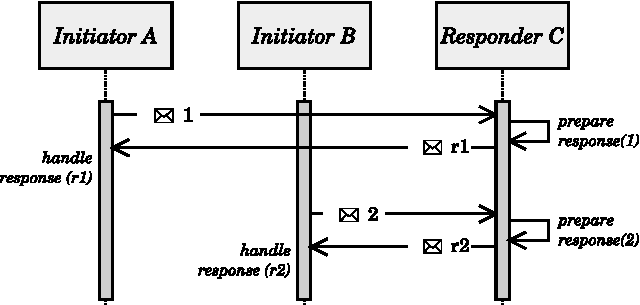
\includegraphics[width=3.0in]{figures/tickExample2.pdf}
	\caption{
		Communication example in JADE. Agents are executed concurrently or in parallel. 
	}
	\label{fig:com-example-jade}
\end{figure}

\begin{figure}
	\centering
	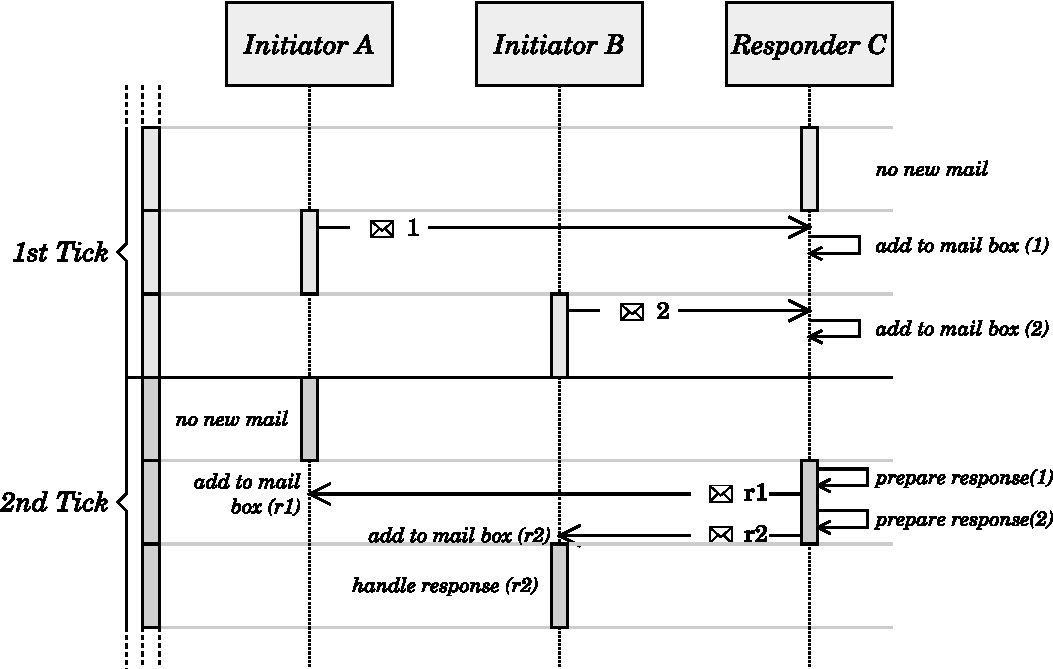
\includegraphics[width=3.8in]{figures/tickExample.pdf}
	\caption{
		Communication example in Repast using \apiname{}.
	}
	\label{fig:com-example-repast}
\end{figure}

While the diagram above represents the agents a scheduled objects, their behaviours are the ones being scheduled. It is worth noting that the order by which Repast executes each scheduled behaviour is unpredictable. In fact, it is not guaranteed that all the behaviours of a single agent are executed consecutively. This is the expected execution when working with Repast as well as with JADE (given its multi-threaded nature) and it is up to the programmer to ensure that the application does not rely on the order of execution.

\subsection{Architecture}

Figure \ref{fig:arch} illustrates the details of \apiname{}'s architecture. Most concepts represented in this diagram are present in JADE, namely the Agent, ACL Message, Behaviour, MTS and DF service.

An agent in \apiname{} contains a MessageQueue and a set of Behaviours. These have access to the agent who owns them and to its MessageQueue. A behaviour that implements an interaction protocol makes use of MessageTemplates. These are used to retrieve relevant messages in each step of the protocol. The MessageTemplates are updated while the protocols go through their different states.

The DFService, as described before, provides the yellow page service. Agents can register or deregister themselves in the DF as well as perform searches. While tasks can be performed during agent setup, in runtime they are typically executed inside Behaviours.

To follow JADE-like communication, ACL Messages carry agent identifiers (AID) for senders and receivers. These AIDs are returned by the DF as search results and are resolved to an agent by the MTS when sending a message. In \apiname{} the MTS keeps a mapping of AIDs to agents for easier access.

The ``plug-in points'' of the API are the Agent, the Behaviour and their derived classes. The API also supports direct access to the DFService. In Figure \ref{fig:arch} all protocol definitions are implied by the generic sub-classes ``ProtocolInitiator'' and ``ProtocolResponder''. 

\begin{figure}[h]
	\centering
	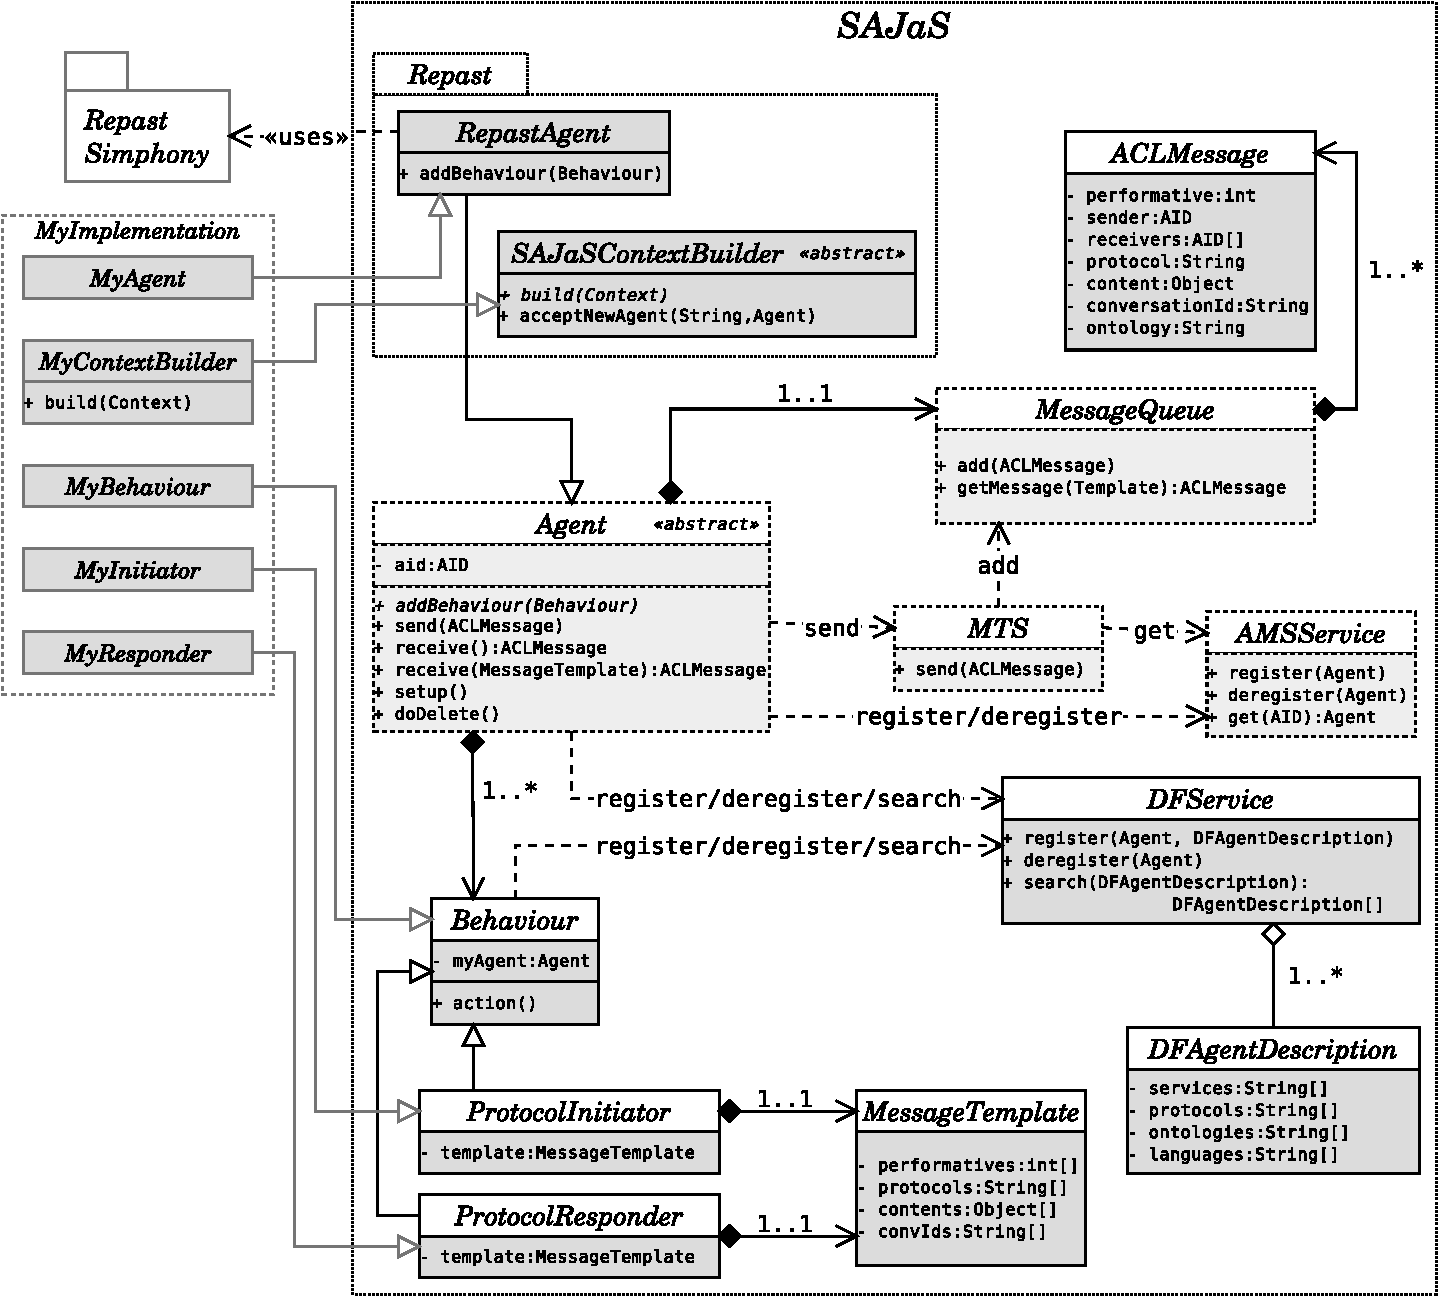
\includegraphics[width=\linewidth]{figures/repacl_arch.pdf}
	\caption{Detailed architecture of \apiname{}. The classes with doted border are internal.}
	\label{fig:arch}
\end{figure}

\subsection{Using Repast}

Even though the API is fairly generic in its architecture, allowing its integration with different frameworks, the main candidate for integration is Repast Simphony. As such, we include an implementation of the AbstractAgent called RepastAgent. It handles the logic of scheduling the behaviour and managing of the Context. The Context is a Repast structure that contains the set of objects to be scheduled. In Figure \ref{fig:arch}, the Context in the API is a wrapper for the Repast Context.


% section proposal (end)
%!TEX root = doc.tex
\section{Validation}
\label{sec:verification}

To perform a validation of the API, we developed a contract net scenario. This is a deterministic test which uses a fixed data set, thus having always the same outcome. The example was implemented in Repast (using \apiname{}) and then manually ported to JADE, after some adaptations.

\subsection{Experimental Setup}

The diagram in Figure \ref{fig:CNetExample} illustrates the contract net created for this test. An agent (the buyer) intends to purchase a certain quantity of three kinds of goods: rice, flour and oats. Besides the quantities of each product it needs, the buyer also stipulates a maximum price for the whole deal. The buyer will issue a call for proposals (CFP) containing a request for supplies to all agents that announce themselves as suppliers in the DF.

Supplier agents have a maximum supply capacity and a price for each product. After receiving a CFP, the supplier will send to the buyer a PROPOSAL containing a price for each product if the demanded supply is within the seller's capacity. Otherwise, a REFUSE message will be sent to the buyer.
Finally, the buyer agent will compare all valid proposals, choose the cheapest offer for each individual product and reply with an ACCEPT PROPOSAL to the best offers, and REJECT PROPOSAL to all others.

\begin{figure}
	\centering
	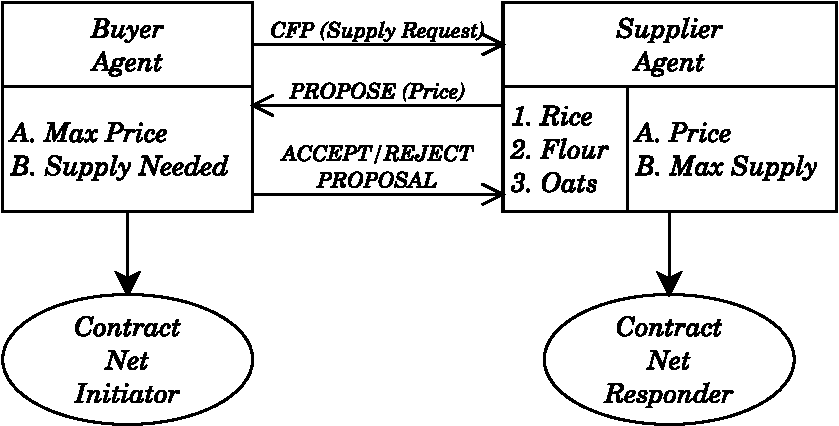
\includegraphics[width=3.0in]{figures/CNetExample.pdf}
	\caption{
		Representation of the example contract net.
	}
	\label{fig:CNetExample}
\end{figure}

Using the same data set with values for prices and supply capacity in both frameworks, we ensured the proper comparison of results. For demonstration purposes, we focused on two simple metrics to evaluate our work: time and outcome. We have run the same experiment with varying numbers of suppliers (as sugested by Figure \ref{fig:performance}) and performed multiple repetitions of each setup.

Time was measured from be begining of the protocol, until all suppliers were notified. The JADE implementation was tested in two different setups: first, with all agents running in a single container; second, with the supplier agents in one container and the buyer in a separate one (but in the same host). In this configuration, all communication between agents happens across containers. All tests were performed using an Intel i7 CPU with 8 logical cores at 2.20 GHz. The second validation metric we used was the actual result of the protocol, i.e who were the supplier agents chosen by the buyer and their price proposals.

\subsection{Results}

For each number of agents, the experiment was run 5 times. The average performance of the experiments is represented in Figure \ref{fig:performance}. As excepted, Repast performance was significantly better, and it excels when the number of agents is high. JADE was able to perform better when using two distinct containers. As studied by Mengistu et. al \cite{mengistu2008scalability}, JADE's performance drops very significantly when there is a high communication-to-computation ratio in the application.

Regarding the outcome of the protocol, as expected the same values were obtained in both implementations, with equal number of suppliers. This allowed us to verify that the behaviour of the protocol is identical in both implementations.


%%%%%%%%%%%%%%%%%%%%%%%%%%%%%%%%%%%%%%%%%%%%%%%
%%%%%%%%%%%%%%%%%% The Chart %%%%%%%%%%%%%%%%%%

\begin{figure}
	\label{fig:performance}
	\centering
	%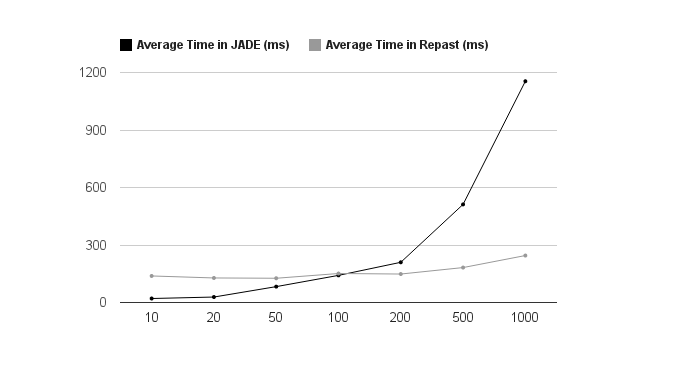
\includegraphics[width=\linewidth]{figures/performance.png}
	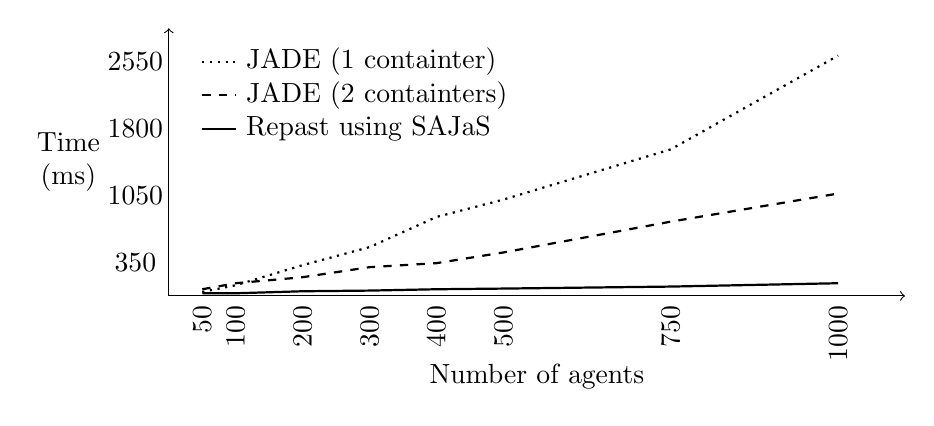
\begin{tikzpicture}[scale=0.85]

		% horizontal axis
		\draw[->] (0,0) -- (11,0);
		\draw (5.5,-1.2) node[align=center] {Number of agents}; %label

		%					  north
		%			west [anchor center] east
		%					  south
		
		% labels
		\draw	(0.5,0) node[rotate=90, anchor=east] {50}
				(1.0,0) node[rotate=90, anchor=east] {100}
				(2.0,0) node[rotate=90, anchor=east] {200}
				(3.0,0) node[rotate=90, anchor=east] {300}
				(4.0,0) node[rotate=90, anchor=east] {400}
				(5.0,0) node[rotate=90, anchor=east] {500}
				(7.5,0) node[rotate=90, anchor=east] {750}
				(10.,0) node[rotate=90, anchor=east] {1000};

		\draw	(-0.5,0.5) node[anchor=center] {350}
				(-0.5,1.5) node[anchor=center] {1050}
				(-0.5,2.5) node[anchor=center] {1800}
				(-0.5,3.5) node[anchor=center] {2550};
		% vertical axis
		\draw[->] (0,0) -- (0,4);
		\draw (-1.5,2) node[align=center] {Time\\(ms)}; %label
		%\draw (-1.5,1.6) node[align=center] {(ms)}; %label

		%% Data %%
		% JADE 2 containers
		\draw[thick,dashed] (0.5,3.0) --
			(1,3.0) node[anchor=west, pos=1.0] {JADE (2 containters)}; %subtitle
		\draw[thick,dashed] (0.5, 0.10) --
					(1.0, 0.19) --
					(2.0, 0.28) --
					(3.0, 0.43) --
					(4.0, 0.49) --
					(5.0, 0.65) --
					(7.5, 1.11) --
					(10., 1.53);
		% JADE 1 containers
		\draw[thick,dotted] (0.5,3.5) --
			(1,3.5) node[anchor=west, pos=1.0] {JADE (1 containter)}; %subtitle
		\draw[thick,dotted] (0.5, 0.06) --
					(1.0, 0.16) --
					(2.0, 0.46) --
					(3.0, 0.73) --
					(4.0, 1.18) --
					(5.0, 1.44) --
					(7.5, 2.19) --
					(10., 3.59);
		% Repast
		\draw[thick] (0.5,2.5) --
			(1,2.5) node[anchor=west, pos=1.0] {Repast using \apiname{}}; %subtitle
		\draw[thick] (0.5, 0.04) --
					(1.0, 0.04) --
					(2.0, 0.07) --
					(3.0, 0.08) --
					(4.0, 0.10) --
					(5.0, 0.11) --
					(7.5, 0.14) --
					(10., 0.19);


	\end{tikzpicture}
	\caption{
		Average execution time of each framework in the different experiments.
	}
\end{figure}

%%%%%%%%%%%%%%%%%%%%%%%%%%%%%%%%%%%%%%%%%%%%%%%
%%%%%%%%%%%%%%%%%%%%%%%%%%%%%%%%%%%%%%%%%%%%%%%

%!TEX root = doc.tex
\section{Future Work}
\label{sec:prototype}

In this section we specify some of the current developments that are making use of \apiname{}, namely a code conversion tool that enables developers proficient in one of the frameworks (Repast or JADE) to port their implementations to the other framework.

\subsection{Conversion Tool Prototype}

The goal of the tool we propose is to allow the automatic conversion of Repast simulations into JADE applications. This conversion tool will not only allow the developer to quickly generate a MAS or create a simulation but also enables a proficient programmer in one framework to quickly get started in developing with the other framework. Figure \ref{fig:prototypeFlow} illustrates these two plausible workflows.

\begin{figure}[h]
	\centering
	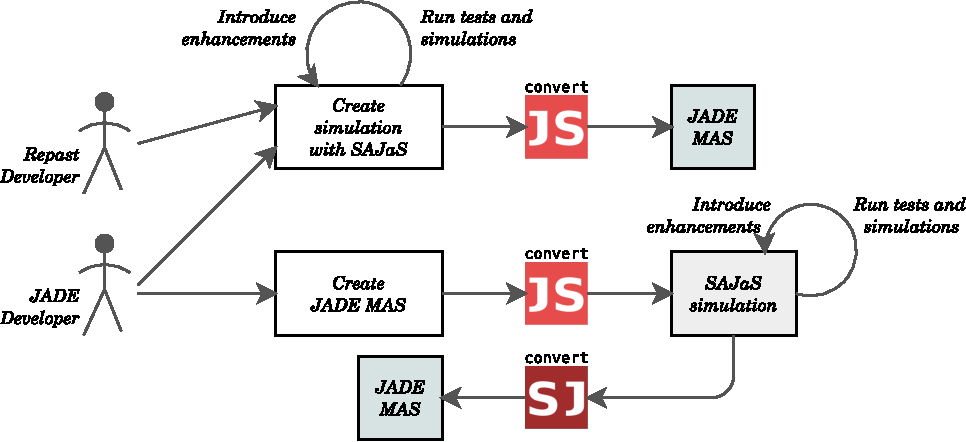
\includegraphics[width=3.0in]{figures/prototypeFlow.pdf}
	\caption{
		Two possible workflows for \apiname{} users
	}
	\label{fig:prototypeFlow}
\end{figure}

The code conversion tool uses the Java Development Tools (JDT) from Eclipse which enables Java programmers to perform introspection and reflection tasks with ease. This approach allows programmers to perform code transformations without having to create parsers for Java code and abstract syntax trees (AST).

The conversion tool will be developed in the form of an Eclipse plug-in, in order to be able to make use of all JDT features.

\subsection{\apiname{} development}

Although \apiname{} is already fit for thed gitevelopment of Repast simulations, it is open to enhancements, namely by enriching it with further missing JADE features. One important trait of \apiname{} is that, although thought for Repast, it is very generic. This means that MABS built using other Java simulation tools can integrate our API successfully in the future and, therefore, use JADE-based features.

%!TEX root = doc.tex
\section{Conclusion}
\label{sec:conclusion}

The development of MAS may require the use of tools that are not readily available in the agent-based framework chosen for the task. The API architecture we propose in this paper emerges as a need to solve a concrete instance of this problem. \apiname{} is our solution to integrating FIPA specifications in MABS frameworks, more specifically Repast, as well as allowing the creation of JADE-like simulations.

The goal of our API is not only to enrich Repast and other simulation frameworks, but also to allow proficient JADE developers in quickly getting started in developing simulations using familiar JADE-based features. \apiname{} also opens the door to MAS to MABS conversion.

The short experiment we described in \ref{sec:verification} showed that our API is capable of handling simulations with a large number of agents, which is common in many simulation scenarios. Aside from the inherent advantages of using open standards in agent systems, \apiname{}'s JADE-based architecture brings Repast closer to JADE. The immediate result of this architecture is that converting models built with Repast using \apiname{} into JADE MAS is very straightforward.

Multiple candidates exist that could have been the object of this paper. JADE and Repast were chosen for their large and active community of researchers, as well as for being open source. One important goal of our project is to eventually release our tools (both \apiname{} and the code conversion tool) for use by the cientific community.


%% comment next 2 commands if numbered appendices are not used
% \appendix
% \chapter{Loren Ipsum} \label{ap1:loren}

Depois das conclusões e antes das referências bibliográficas,
apresenta-se neste anexo numerado o texto usado para preencher a
dissertação.

\section{O que é o \emph{Loren Ipsum}?}

\emph{\textbf{Lorem Ipsum}} is simply dummy text of the printing and
typesetting industry. Lorem Ipsum has been the industry's standard
dummy text ever since the 1500s, when an unknown printer took a galley
of type and scrambled it to make a type specimen book. It has survived
not only five centuries, but also the leap into electronic
typesetting, remaining essentially unchanged. It was popularised in
the 1960s with the release of Letraset sheets containing Lorem Ipsum
passages, and more recently with desktop publishing software like
Aldus PageMaker including versions of Lorem Ipsum~\citep{kn:Lip08}. 

\section{De onde Vem o Loren?}

Contrary to popular belief, Lorem Ipsum is not simply random text. It
has roots in a piece of classical Latin literature from 45 BC, making
it over 2000 years old. Richard McClintock, a Latin professor at
Hampden-Sydney College in Virginia, looked up one of the more obscure
Latin words, consectetur, from a Lorem Ipsum passage, and going
through the cites of the word in classical literature, discovered the
undoubtable source. Lorem Ipsum comes from sections 1.10.32 and
1.10.33 of ``de Finibus Bonorum et Malorum'' (The Extremes of Good and
Evil) by Cicero, written in 45 BC. This book is a treatise on the
theory of ethics, very popular during the Renaissance. The first line
of Lorem Ipsum, ``Lorem ipsum dolor sit amet\ldots'', comes from a line in
section 1.10.32.

The standard chunk of Lorem Ipsum used since the 1500s is reproduced
below for those interested. Sections 1.10.32 and 1.10.33 from ``de
Finibus Bonorum et Malorum'' by Cicero are also reproduced in their
exact original form, accompanied by English versions from the 1914
translation by H. Rackham.

\section{Porque se usa o Loren?}

It is a long established fact that a reader will be distracted by the
readable content of a page when looking at its layout. The point of
using Lorem Ipsum is that it has a more-or-less normal distribution of
letters, as opposed to using ``Content here, content here'', making it
look like readable English. Many desktop publishing packages and web
page editors now use Lorem Ipsum as their default model text, and a
search for ``lorem ipsum'' will uncover many web sites still in their
infancy. Various versions have evolved over the years, sometimes by
accident, sometimes on purpose (injected humour and the like). 

\section{Onde se Podem Encontrar Exemplos?}

There are many variations of passages of Lorem Ipsum available, but
the majority have suffered alteration in some form, by injected
humour, or randomised words which don't look even slightly
believable. If you are going to use a passage of Lorem Ipsum, you need
to be sure there isn't anything embarrassing hidden in the middle of
text. All the Lorem Ipsum generators on the Internet tend to repeat
predefined chunks as necessary, making this the first true generator
on the Internet. It uses a dictionary of over 200 Latin words,
combined with a handful of model sentence structures, to generate
Lorem Ipsum which looks reasonable. The generated Lorem Ipsum is
therefore always free from repetition, injected humour, or
non-characteristic words etc. 


%%----------------------------------------
%% Final materials
%%----------------------------------------

%% Bibliography
%% Comment the next command if BibTeX file not used
%% bibliography is in ``myrefs.bib''
\PrintBib{myrefs}
%\bibliography{myrefs}

%% Index
%% Uncomment next command if index is required
%% don't forget to run ``makeindex pdis-en'' command
%\PrintIndex

\end{document}
